\documentclass[11pt,a4paper]{scrartcl}
\usepackage[T1]{fontenc}
\usepackage{microtype}
\usepackage{lmodern}
\usepackage{amsmath}
\usepackage{amsfonts}
\usepackage{amssymb}
\usepackage{enumerate}
\usepackage{graphicx}
\usepackage{float}


\def\ojoin{\setbox0=\hbox{$\bowtie$}%
  \rule[-.02ex]{.25em}{.4pt}\llap{\rule[\ht0]{.25em}{.4pt}}}
\def\leftouterjoin{\mathbin{\ojoin\mkern-5.8mu\bowtie}}
\def\rightouterjoin{\mathbin{\bowtie\mkern-5.8mu\ojoin}}
\def\fullouterjoin{\mathbin{\ojoin\mkern-5.8mu\bowtie\mkern-5.8mu\ojoin}}

\begin{document}

\author{Johannes Merkle\\Ralf Vogler}
\title{Query Optimization}
\subtitle{4. Exercise}

\maketitle

\section*{Exercise 1}

\subsection*{1}

\begin{figure}[H]
	\begin{center}
		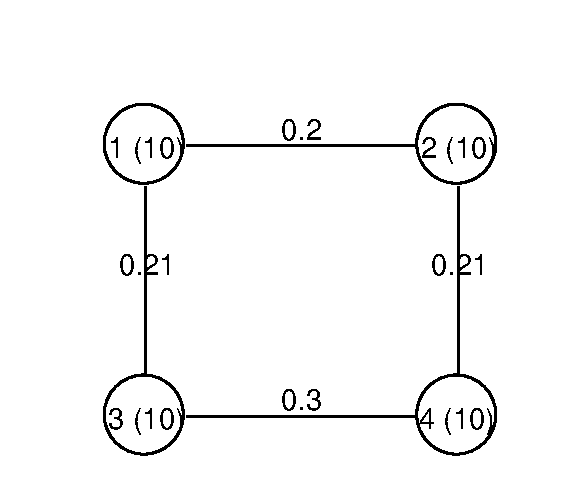
\includegraphics{graphs/querygraph}
	\end{center}
	\caption{Query graph. The number in brackets denotes the cardinality}
	\label{fig:qg}
\end{figure}
	
\begin{figure}[H]
	\begin{center}
		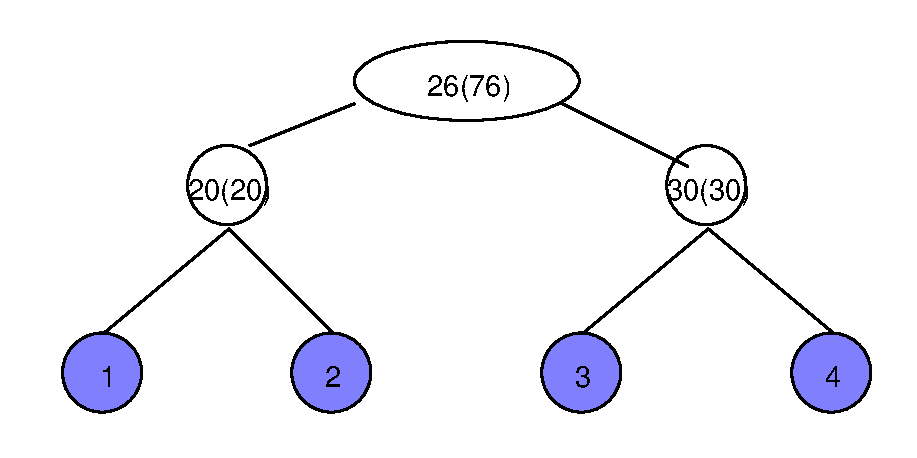
\includegraphics{graphs/goo}
	\end{center}
	\caption{The join tree produced by the GOO algorithm. Blue nodes are the relations. The white nodes are the joins. The number in front of the brackets denotes the cardinality. The number in brackets denotes $C_{out}$ of the subtree. $C_{out}$ of the full join tree is 76.}
	\label{fig:goo}
\end{figure}

\begin{figure}[H]
	\begin{center}
		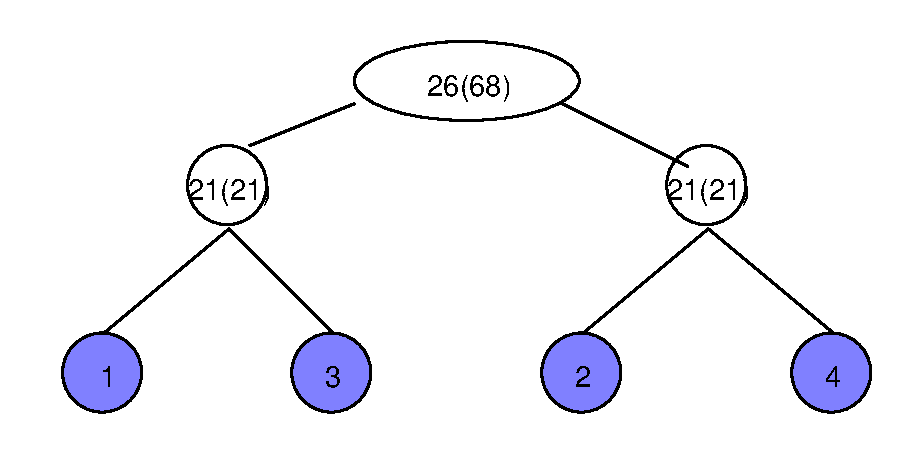
\includegraphics{graphs/optimal}
	\end{center}
	\caption{The optimal join tree. Blue nodes are the relations. The white nodes are the joins. The number in front of the brackets denotes the cardinality. The number in brackets denotes $C_{out}$ of the subtree. $C_{out}$ of the full join tree is 68.}
	\label{fig:optimal}
\end{figure}
	

\subsection*{2}

We only need to construct $G^P_1$ and $G^P_3$ as relations 2 and 4 are similar to relations 1 and 3 in terms of the result of the algorithm (up to renaming of the relations).

\begin{figure}[H]
	\begin{center}
		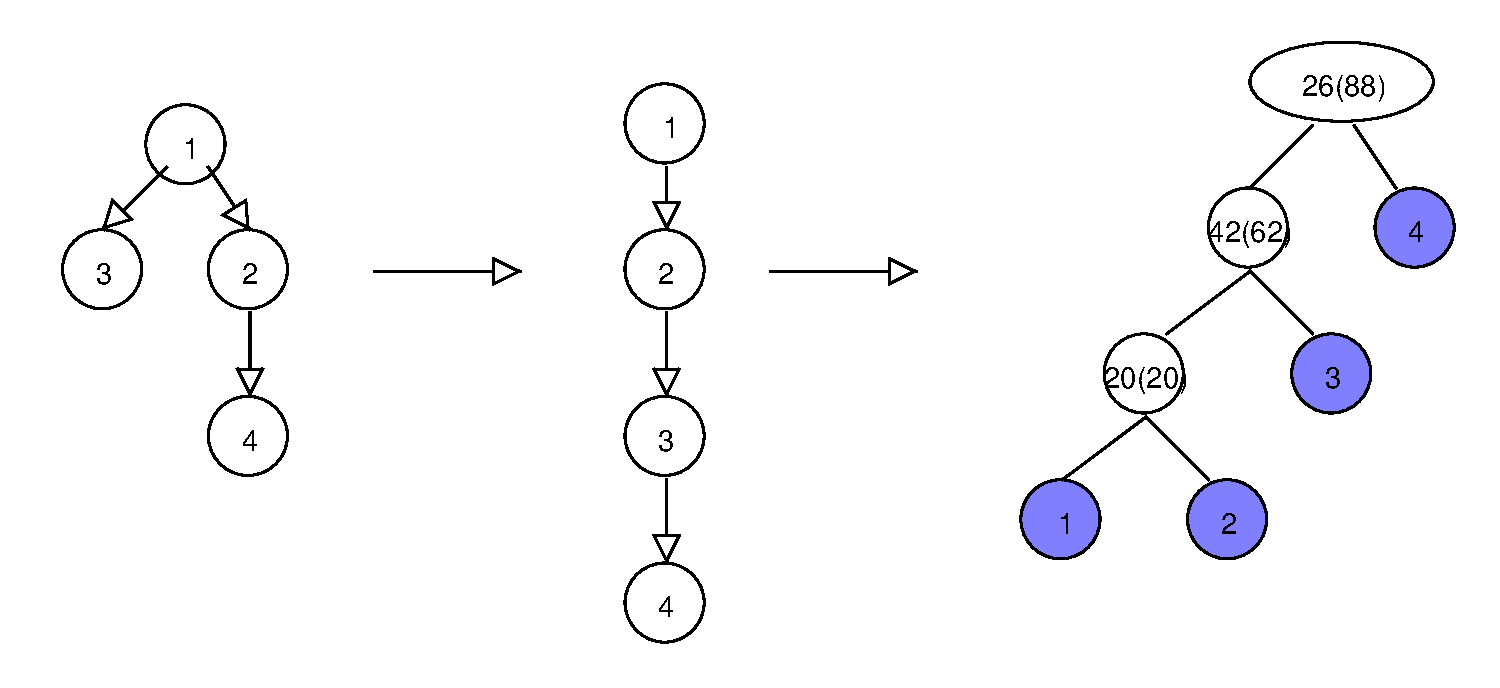
\includegraphics[width=\textwidth]{graphs/gp1}
	\end{center}
	\caption{$G^P_1$. The first tree shows the initial tree after removing the cycle by creating the minimum spanning tree. We can't normalize at this point because $rank(2)<rank(4)$. In the next step we merge the subtrees because $rank(2)<rank(3)$. The last tree is the resulting join tree with a resulting $C_{out}$ of 88}
	\label{fig:gp1}
\end{figure}

\begin{table}[H]
  \caption{Values for $G^P_1$}
  \begin{center}
 \begin{tabular}{c|c|c|c|c|c}
  relation & n & s & C & T & rank\\
  \hline 
  2 & 10 & 0.2 & 2 & 2 & $\frac{1}{2}$ \\
  3 & 10 & 0.21 & 2.1 & 2.1 & $\frac{1.1}{2.1}$ \\
  4 & 10 & 0.21 & 2.1 & 2.1 & $\frac{1.1}{2.1}$ \\
 \end{tabular}  
  \end{center}
 \label{tab:gp1}
\end{table}

\begin{figure}[H]
	\begin{center}
		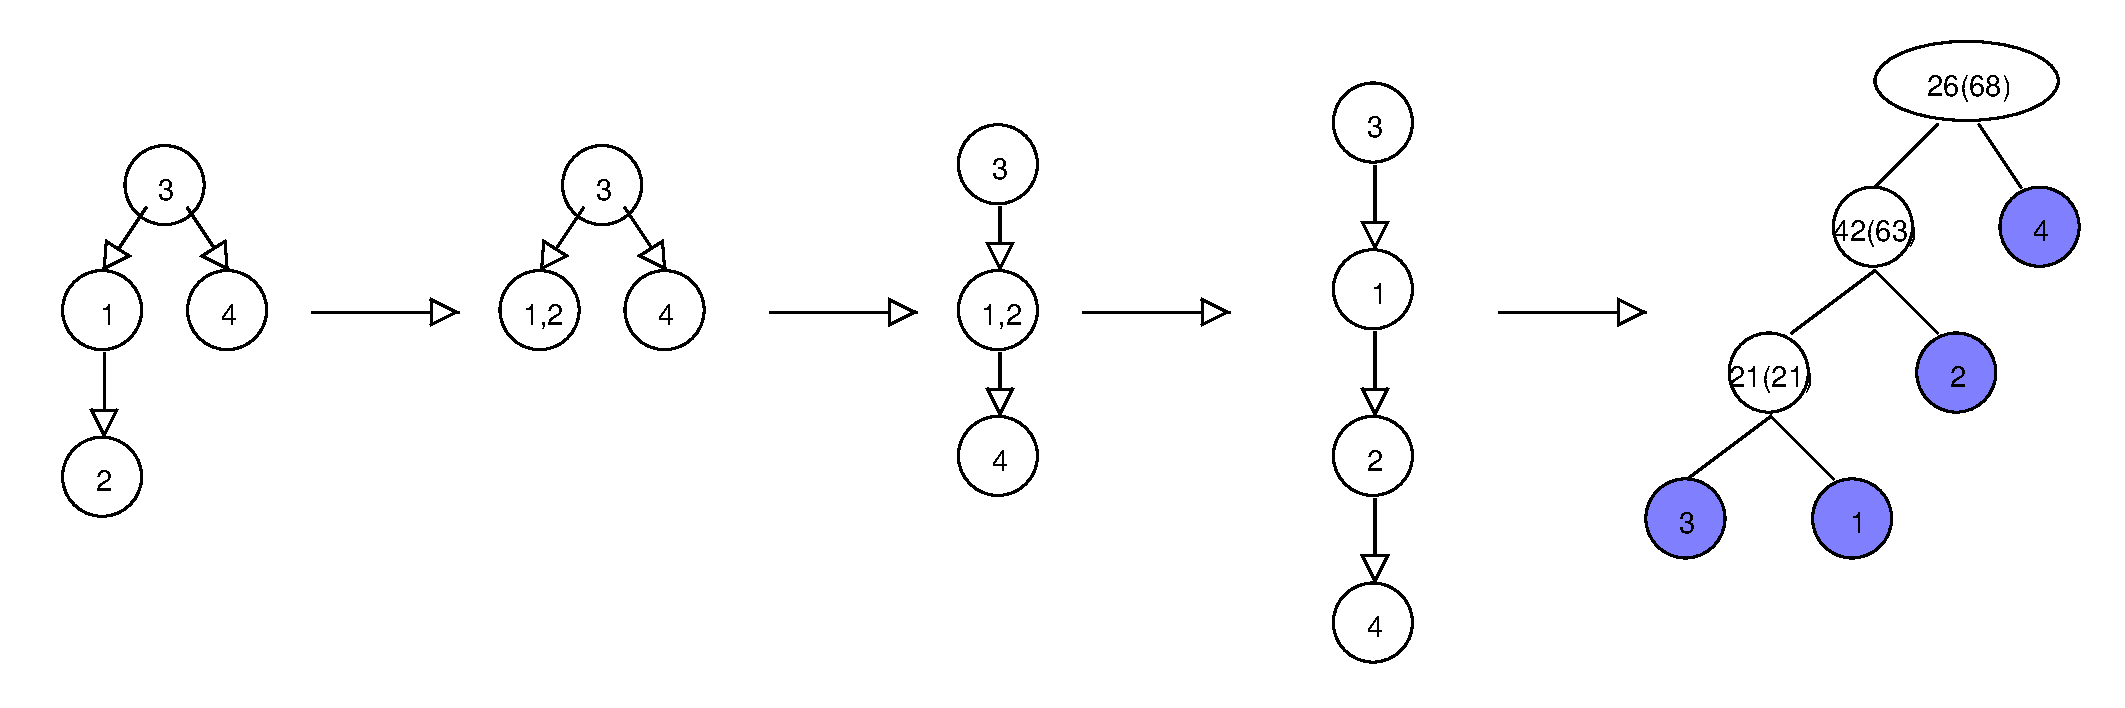
\includegraphics[width=\textwidth]{graphs/gp3}
	\end{center}
	\caption{$G^P_3$. The first tree shows the initial tree after removing the cycle by creating the minimum spanning tree. In the next step we normalize the subtree because $rank(1)>rank(2)$. Then we merge the subtrees because $rank(1,2)<rank(4)$ and after that we can denormalize the tree. The last tree is the resulting join tree with a resulting $C_{out}$ of 68. We see that the IKKBZ heuristics are not optimal either and in this case result in even worse costs than the GOO algorithm.}
	\label{fig:gp3}
\end{figure}

\begin{table}[H]
  \caption{Values for $G^P_3$}
  \begin{center}
 \begin{tabular}{c|c|c|c|c|c}
  relation & n & s & C & T & rank\\
  \hline 
  1 & 10 & 0.21 & 2.1 & 2.1 & $\frac{1.1}{2.1}$ \\
  2 & 10 & 0.2 & 2 & 2 & $\frac{1}{2}$ \\
  4 & 10 & 0.3 & 3 & 3 & $\frac{2}{3}$ \\
  1,2 & 20 & 0.21 & 6.3 & 4.2 & $\frac{3.2}{6.3}$ \\
 \end{tabular}  
  \end{center}
 \label{tab:gp1}
\end{table}

\section*{Exercise 2}

see folder tinydb

\end{document}
